\chapter{Design}

This chapter contains a high level description of the design choices made in the process of creating Viskell.
The specific implementation details are discussed in chapter \ref{chap:implementation} on page \pageref{chap:implementation}.

\section{User interface}

\subsection{Graphical design}

The entire user interface consists of a number of components floating around on a drag and drop canvas.

\subsubsection{Blocks and lines}
Blocks and the way they are connected with lines defines the Haskell program. We chose blocks since this is a familiar element for users. In Haskell, values are passed to functions without being saved as variables. The lines between blocks represent this flow. Thus, a program can be built like an electronic circuit. In this abstraction the blocks can be seen as small calculators or computer chips while the lines are copper wires which carry the data.

Blocks have input and output anchors that can be used to create connections from one block to another, essentially representing the Haskell program flow. Input anchors are positioned on the top of a block, the output anchor on the bottom side. The inside of a block is defined by the block itself, for functions this is a name and the types of the arguments it expects.

We chose to make a distinction between three kinds of blocks, each having their own colour to make them easily recognizable.
The first kind is an output block, which represents a constant value. \index{value block} \index{output block}
This input block can be connected to other blocks which can use its outputted value as input.
Besides the most basic output block, which is the value block that takes a string as input for creation and then automatically detects the type, there is also a slider available. \index{slider block}

The second kind of block displays the program's output. \index{input block}
There are multiple versions, ranging from a simple block that displays the string representation of its input to a graph block which can show the curve of a function. \index{graph block}

The third kind of block is a function block. This block has a number of inputs, a single output, and a knot defining the number of inputs that need to be connected. \index{function block}
The number of inputs can be changed by moving the knot left or right over the function's arguments.
This allows for passing (partially applied) functions as input for other functions. \index{partial application}
A useful example for this is the \code{map} function.

During the project, many different ideas where pitched for blocks. Eventually we went with something a bit different from the client's initial idea. Some more information about this can be found in chapter \ref{chap:Evaluation}.

\begin{figure}[p]
	\centering
	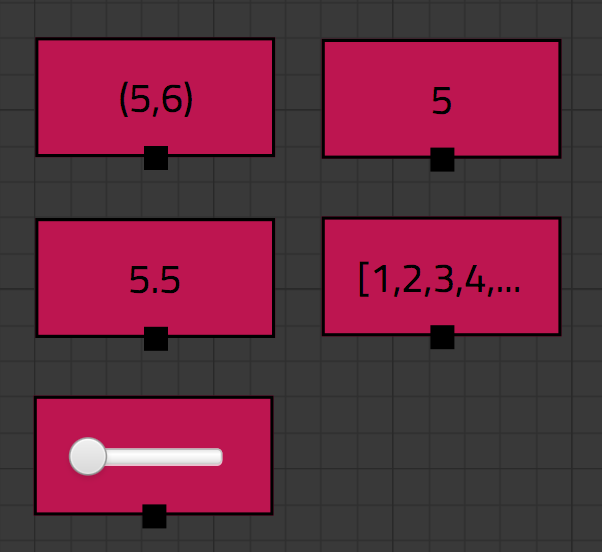
\includegraphics[scale=0.5]{Images/blocks-inputs}
	\caption{Different input blocks}
	\label{fig:blocks-inputs}
\end{figure}

\begin{figure}[p]
	\centering
	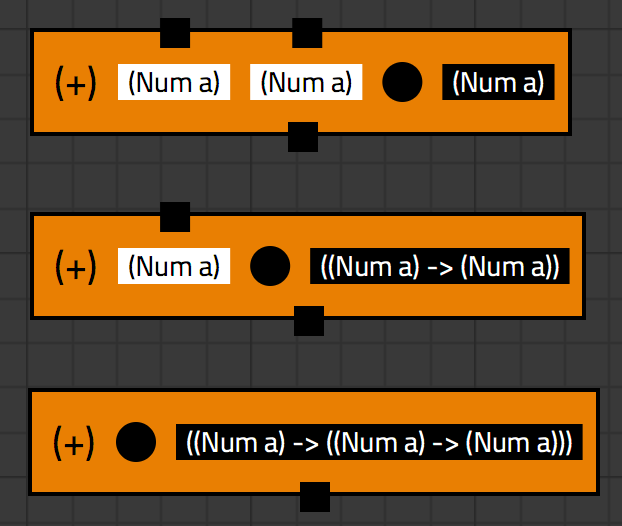
\includegraphics[scale=0.5]{Images/blocks-bowties}
	\caption{Partial application of functions}
	\label{fig:blocks-bowties}
\end{figure}

\begin{figure}[p]
	\centering
	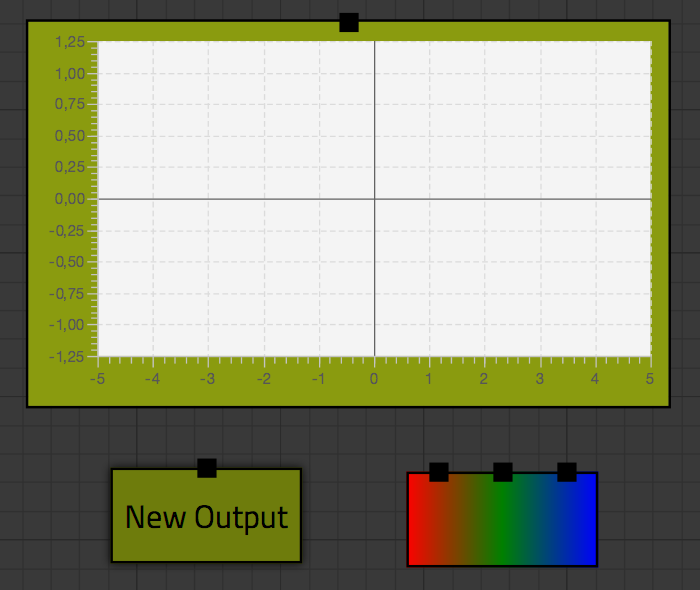
\includegraphics[scale=0.5]{Images/blocks-outputs}
	\label{fig:blocks-outputs}
\end{figure}

\begin{figure}[p]
	\centering
	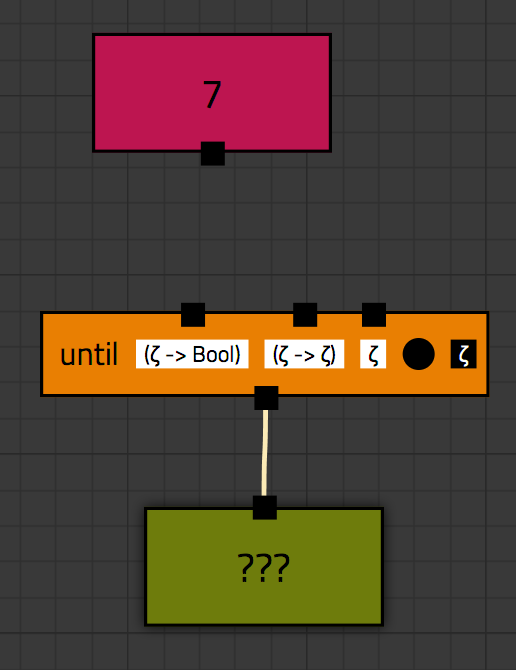
\includegraphics[scale=0.5]{Images/blocks-example}
	\caption{Different kinds of blocks}
	\label{fig:blocks-example}
\end{figure}

\subsubsection{Errors}

An important part of Viskell is representing programming errors.
Instead of requiring users to stop editing and compile a complete program, Viskell performes type checking whenever a change in the program is made. Due to this strategy, type errors can be displayed as soon as a user connects two blocks. These errors are represented as a coloured, red, line and coloured, red, type in the target block's input arguments. An icon is displayed inside the incorrectly connected anchor as well to help colour blind users.

\subsubsection{Menus}

During the design process many ideas for the menus came up.
One of the first ideas was to have a circular menu. \label{circular_menu} \index{circle menu}
The advantages of the circular menu would be that the orientation of the device would not have any influence on the usability of the menu.
This would makes using the program on a large multi-touch table with multiple users easier.
However, the implementation of the menu would take too much time and on top of that the client preferred something more like his initial sketches. The idea of a circular menu was therefore dropped.

\begin{figure}[p]
	\centering
	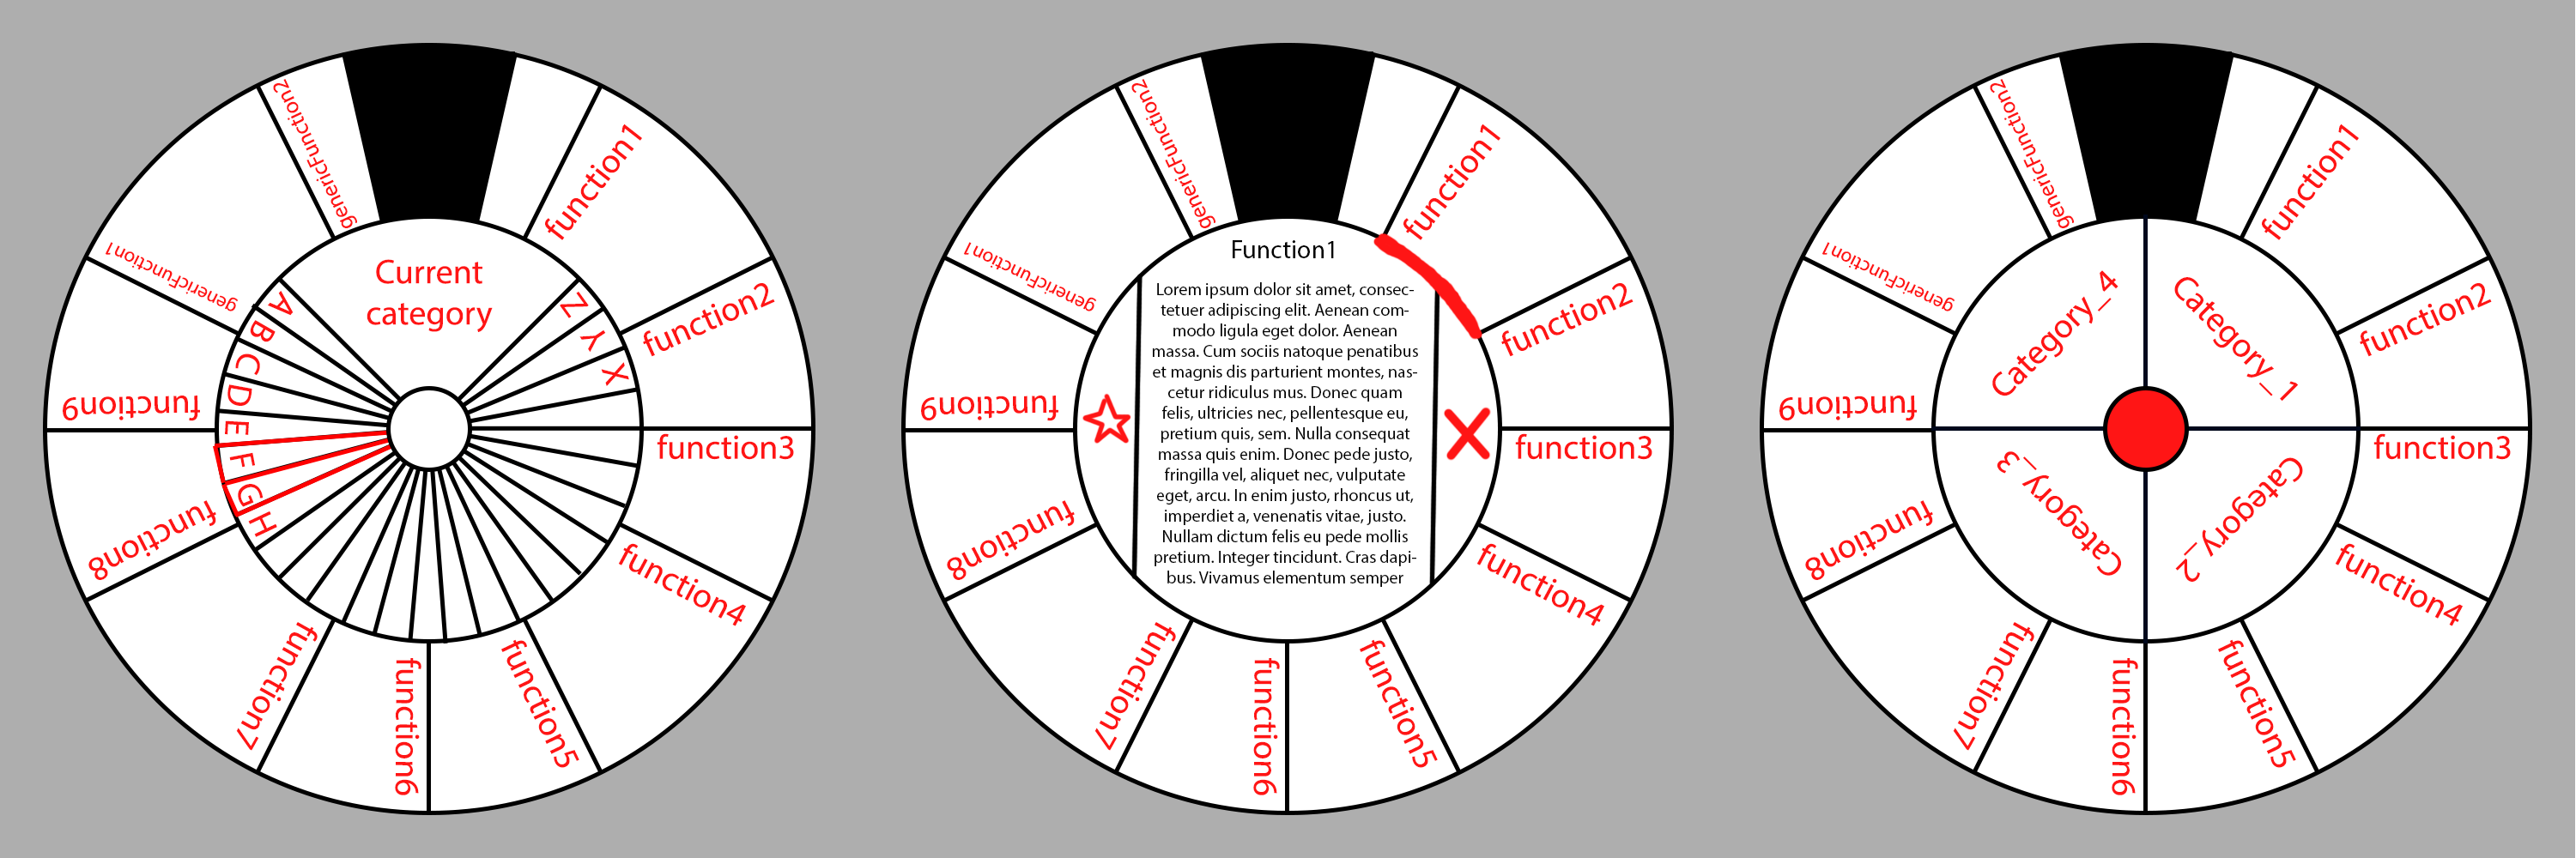
\includegraphics[width=\textwidth]{Images/circlary}
	\caption{Concept of circular menu}
	\label{fig:circlary}
\end{figure}
\begin{figure}[p]
	\centering
	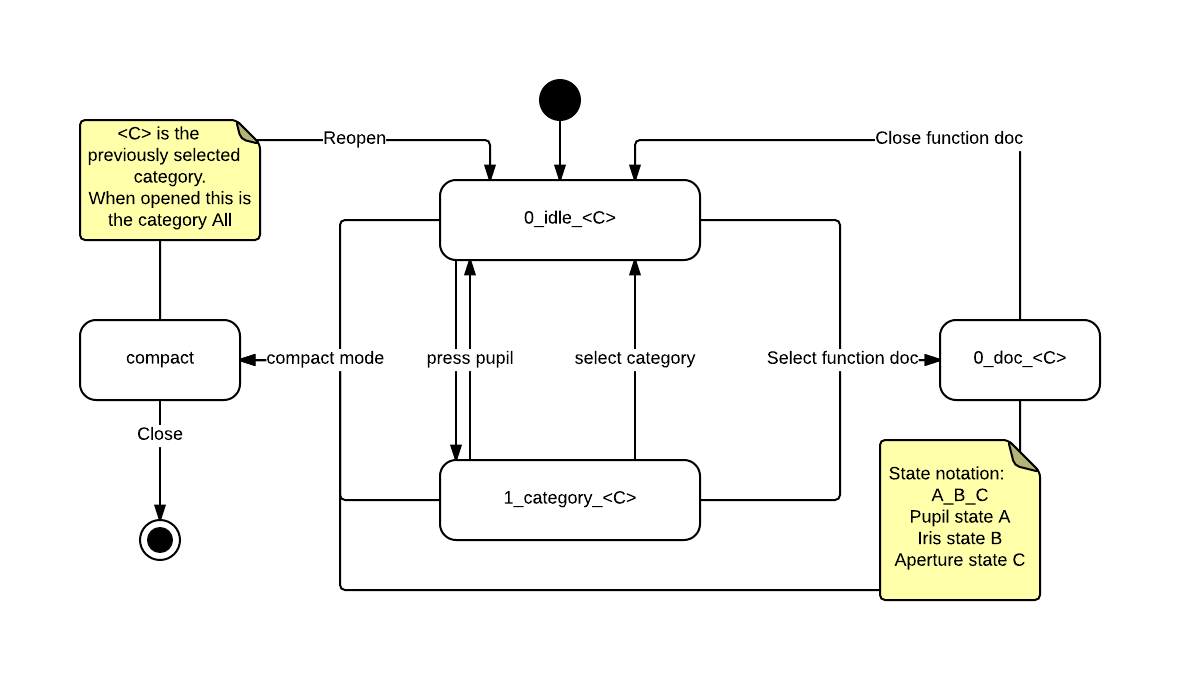
\includegraphics[scale=0.5]{Images/diagram-circlary}
	\caption{Circular menu diagram}
	\label{fig:diagram-circlary}
\end{figure}

The final menu design has two separate menus, one for adding new blocks and one for contextual options on existing blocks.

The primary menu (or `function menu') uses `drawers' for the categories of the functions. \index{primary menu} \index{function menu}
This way it is easy to find functions even without an extensive knowledge of Haskell.
In- and output blocks and the function definition block can be created using buttons at the bottom of the menu.
This location is chosen to make them quickly available.
The primary menu can be opened multiple times at once and moved around the screen so multiple users can work on a single program. An additional benefit of having a floating menu is that the physical size of a screen never impacts reachability of the menu, as opposed to having a menu stuck to one of the sides.

\begin{figure}[p]
	\centering
	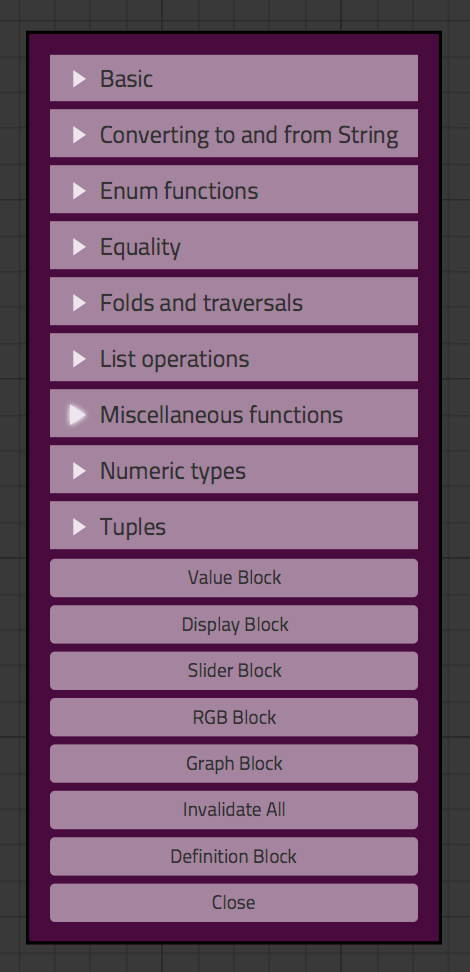
\includegraphics[scale=0.5]{Images/menu}
	\caption{Primary menu}
	\label{fig:ui-menu}
\end{figure}

The context menu is compact so is does not take up too much space. \index{context menu}
It contains clear icons which represent different actions for the single selected block, like delete.
The icons are large enough to touch, even for people with large fingers.

\begin{figure}[p]
	\centering
	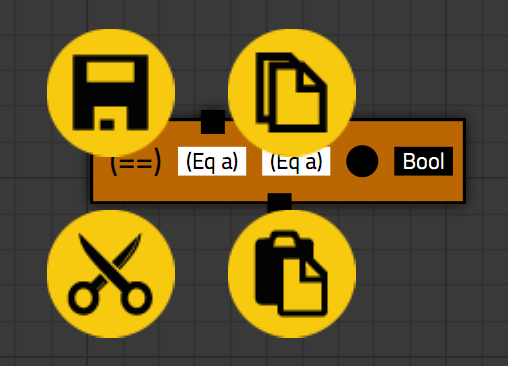
\includegraphics[scale=0.5]{Images/blocks-menu}
	\caption{Context menu}
	\label{fig:blocks-menu}
\end{figure}

\subsubsection{Colour scheme}

The background colour of the canvas is a shade of dark grey.
This is chosen because it is less tiring for the eyes than white and allows for a high contrast.
The background also incorporates a grid pattern so users can align elements on the screen if they like to.

All other components feature a cheerful colour scheme.
This colour scheme provides good contrast with the background and solid recognizability for the different kinds of blocks.

\subsection{Behaviour and interaction design}

Our goal was to provide an easy to use and intuitive (multi-)touch interface, with a very flat learning curve. To achieve this we looked at the way smart phones provided touch interaction and tried to stick to their philosophy on the matter.

A very clear rule in that philosophy is to always have to perform as little actions as possible. We strived to achieve this with Viskell. An example of this is the ability to edit a connection. Instead of having to delete a connection before create a new one we added the ability to `overwrite' it. This combines what would otherwise be two separate actions into a single action. Our menus were also constructed with the same goal in mind.

To make sure that the user has a good overview of what he is doing we focussed on good, instantaneous feedback. This can be seen in the way a type mismatch is displayed. Besides this users should also be able to correct the error quickly, for example with an undo button or the ease with which a connection is changed.

An activity diagram of the interaction a user can have with Viskell is shown in figure \ref{fig:activitydiagram} on page \pageref{fig:activitydiagram}. As can be seen in the figure, the number of actions a user can perform is not very large. This confirms the short learning curve we wanted to achieve. Although the number of actions is not very large, the number of possibilities in the program at a given point is quite extensive. This is visualised by the many lines in the activity diagram.

\begin{figure}[p]
	\centering
	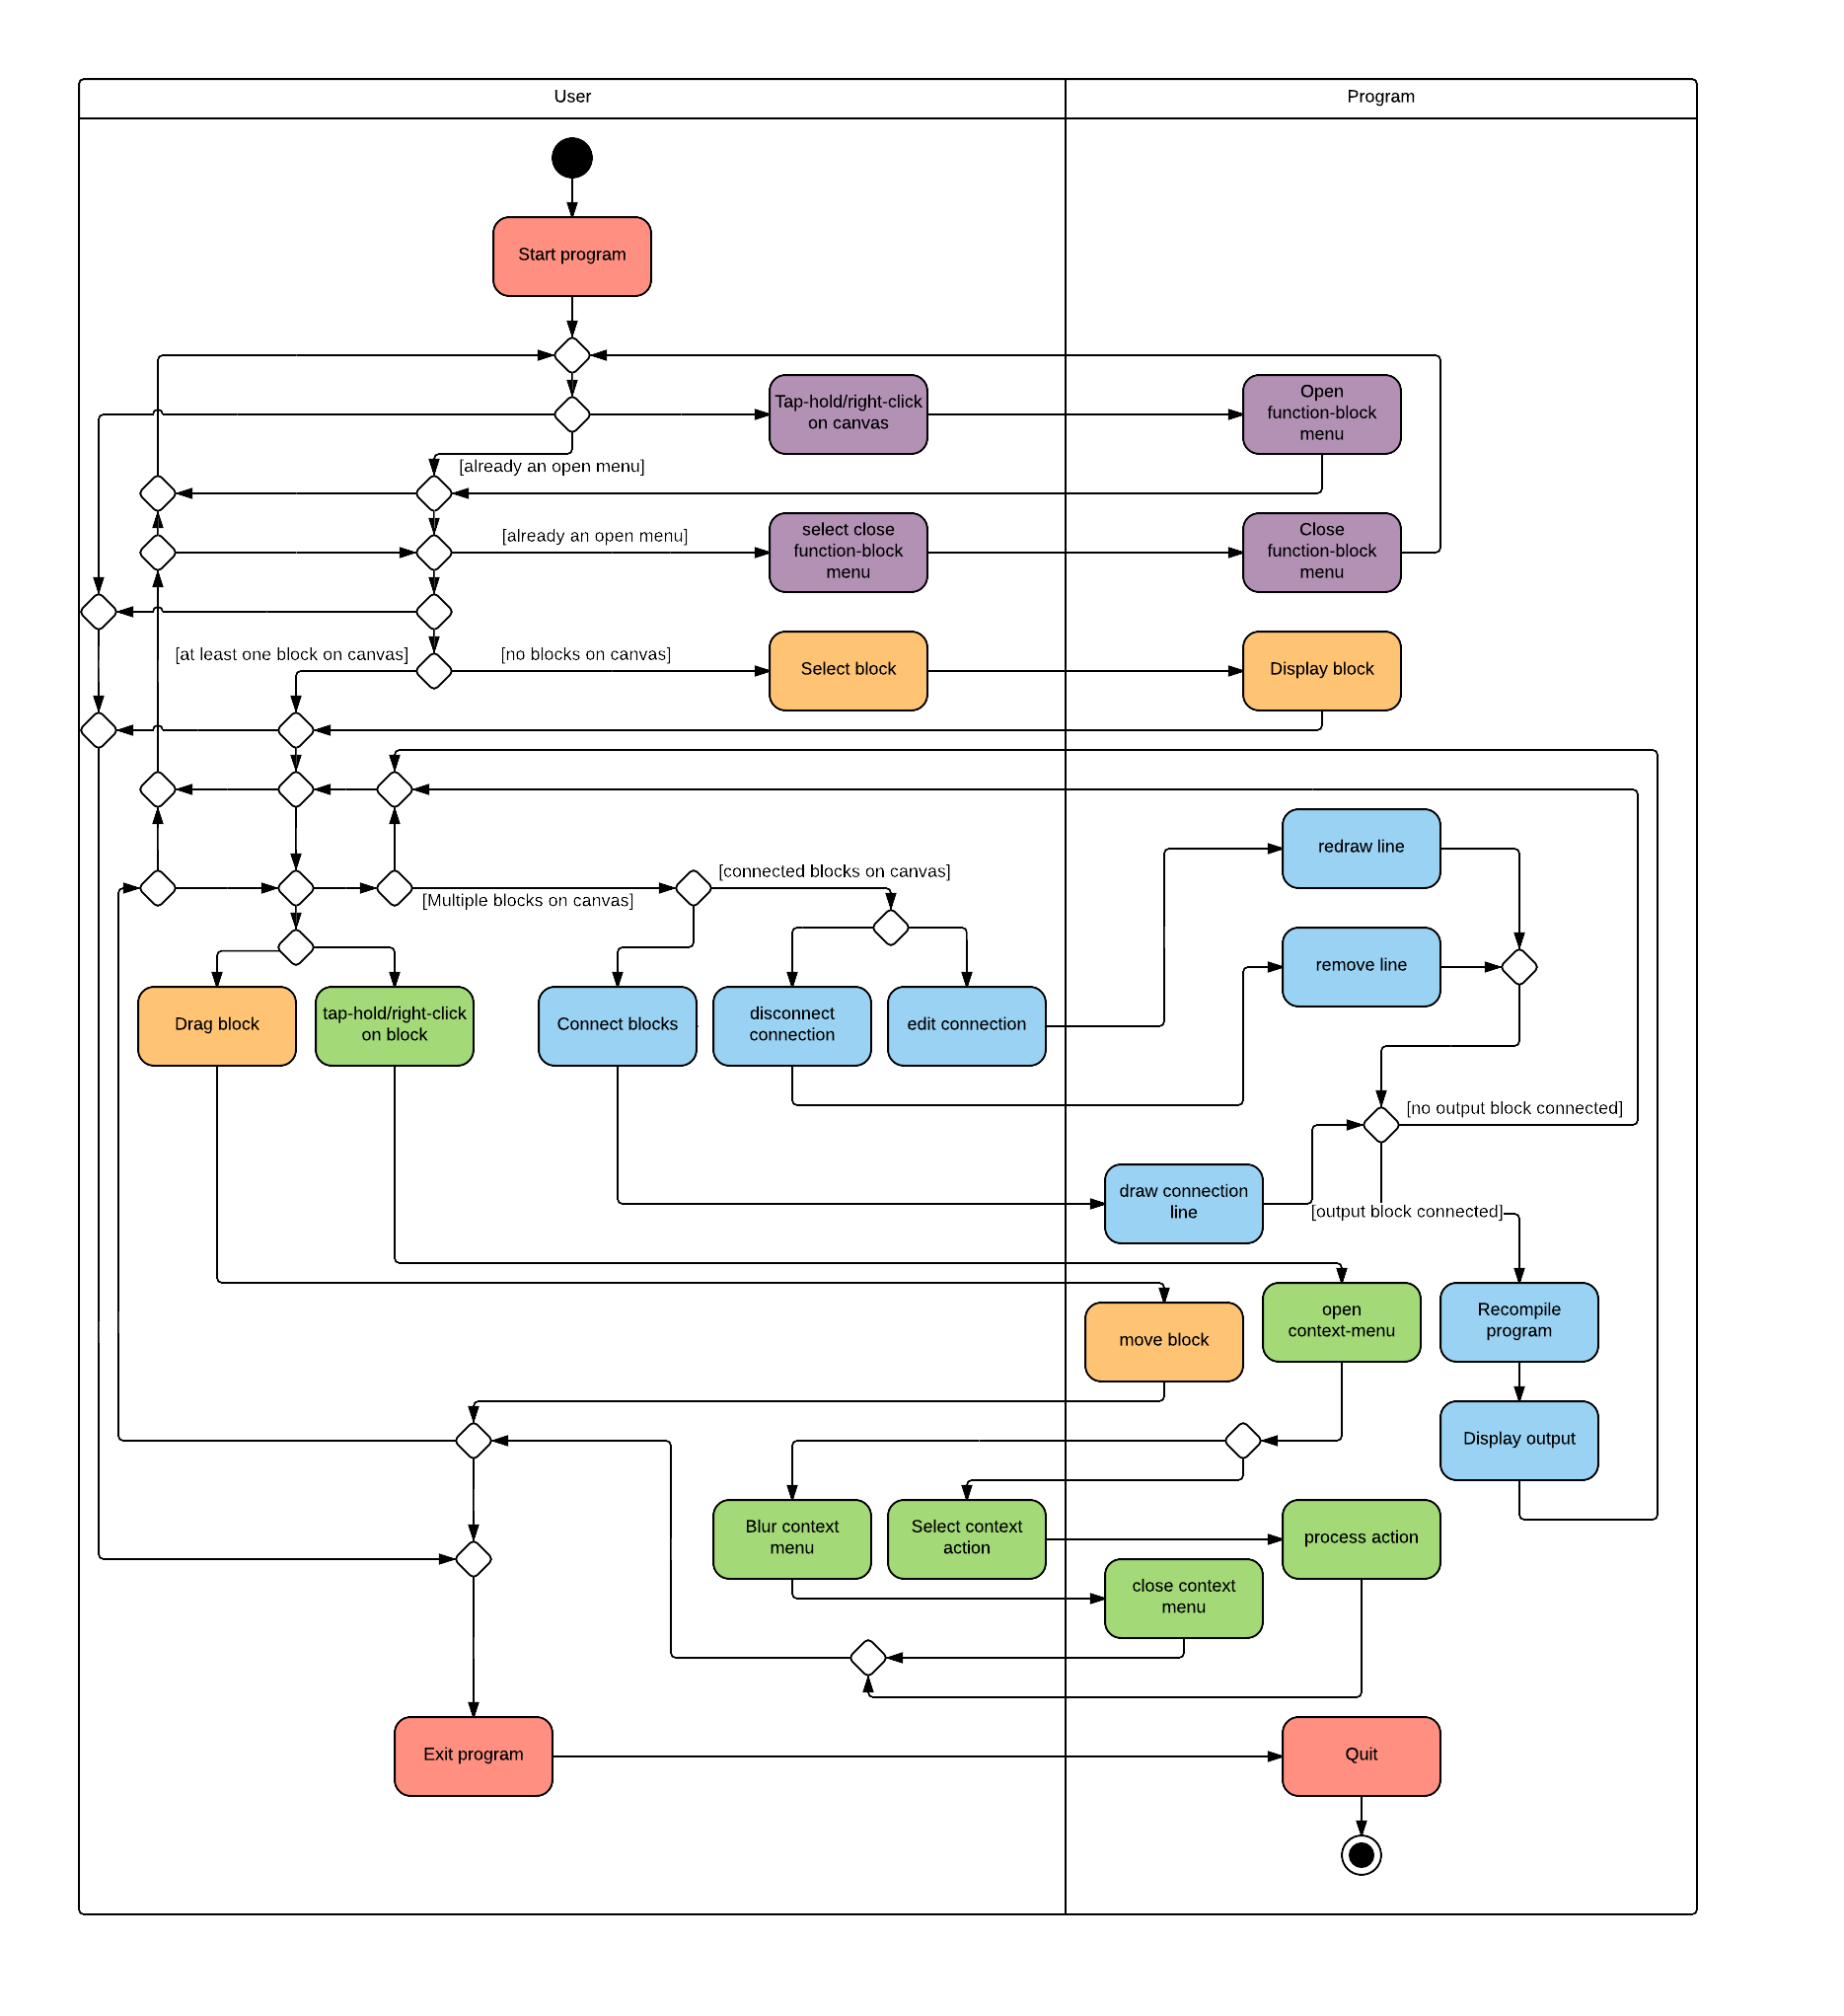
\includegraphics[width=\textwidth]{Images/activitydiagram}
	\caption{Activity diagram}
	\label{fig:activitydiagram}
\end{figure}

The fact that it is possible to almost do anything from any state of the program is probably a (positive) side effect of our goals regarding multi-touch support. While the client's suggestions on the matter were a bit vague, we eventually settled on the requirement that all single user actions needed to be able to be concurrently performed by multiple users. This resulted in almost all actions being able to happen concurrently. Despite our attempts, some actions still do not support multi-touch, for example opening a function menu, yet this should be relatively easy to solve in the future.

\section{Languages and libraries}
Viskell is written in Java 8, which comes bundled with JavaFX. \index{JavaFX}
Java 8 is chosen because it, unlike Java 7, still receives public updates at the moment of writing and allows us to make use of some of the new features in this version.

Viskell uses TactileFX, a JavaFX touch screen library developed at the University of Twente.
The client wanted the program to use this library, which also means that Viskell had to use Java and JavaFX.

Furthermore, the following libraries have been used:

\begin{itemize}
	\item Antlr 4 (\url{http://www.antlr.org/})
	\item Guava (\url{https://github.com/google/guava})
	\item JFXtras (\url{http://jfxtras.org/})
\end{itemize}

\section{High-level architecture}
Viskell consists of two parts, a front end and a back end. \index{front end} \index{back end}
The front end is responsible for providing a user interface, handling user input, displaying error messages, and communicating with the back end.
The back end consists of a representation for Haskell code in Java, an interface to GHCi (see \ref{GHCi} on page \pageref{GHCi}) and functionality to make working with the back end easier.
This separation is made to make development and debugging easier.
It also makes using the user interface for a different purpose a bit easier, although the user interface has been designed specifically for our use case.

\section{Front end architecture}
We designed Viskell with multi-touch interfaces in mind. \code{\gls{TactileAPI}}, an extension for JavaFX, was made available to us to assist with multi-touch interfacing.

\code{CustomUIPane}, our extension of \code{TactilePane}, has many of the same responsibilities of a main \code{Window} and stores most of the program state.
Listeners are attached to the \code{CustomUIPane} instance to monitor mouse and touch events that are directly responsible for the interaction with menus.

While the general listeners are controlled from the \code{CustomUIPane}, components often have specific listeners attached to them.
This is done to allow the gestures to easily change the state of the a component. Complex handlers were given their own class where possible.

Different components are placed on the \code{CustomUIPane}. All of the components make use of the FXML markup language of JavaFX.

\subsection{Gestures}
Interaction with the user interface is possible with touch gestures on the touch screen or by using a mouse. Since JavaFX only supports three different multi-touch events (pressed, moved and released), we had no choice but to base as much as possible of the interaction on these three events. Equivalent mouse events are used to preserve symmetry and ease development on systems without touch screens. Some more advanced mouse gestures are used (for example when opening menus), these can be accessed with touch from synthesized touch events. However, these more advanced gestures do not work correctly with multi-touch.

\subsection{Components}
All elements that are placed on the canvas are a component of some kind.
Each component is an extension of a JavaFX \code{Node}. This is done in order to be able to directly link interactivity to the objects that are visible on the screen.

Components can be categorized in four classes: blocks, anchors, lines and menus.
Blocks can be further categorized into function blocks, input blocks and output blocks.

The term `input blocks' is used here for blocks that can receive input, and `output blocks` is used for blocks that provide output. There is are interfaces for both kinds, these can be implemented by a \code{Block}. The \code{DisplayBlock} class is an example of an input block, the \code{ValueBlock} class is an example of an output block. Function blocks implement both interfaces.

\subsection{FXML \& CSS}
FXML is used in an attempt to separate structure from behaviour. This separation turned out to be very hard to keep. The end result is that FXML is used to construct most components while the code adds or changes the component after it has been built from FXML. FXML was used to set most of the UI settings like height, width and other attributes.

CSS is used to separate style from structure. This separation turned out to be easier to keep. We defined the visual look (such as colours) of the entire UI in style classes in a single CSS file. Fitting style classes are applied to each component, mostly using FXML. Some style classes are updated dynamically (such as the error style class), this is done in Java.

\section{Back end architecture}

A result of our design choices is that our Java program needs to have a basic understanding of the Haskell programming
language. For this purpose we implemented two tree structures - one for expressions, one for types - supported by an
interface for GHCi, a type signature parser and a catalog.

\subsection{Communication with GHCi}
\label{GHCi}
\index{GHCi}

The base of the back end is an interface for communication with GHCi. This interface allows us to run Haskell code
generated by the users of our application. As implementing a complete type checker for Haskell is a major challenge this
interface can also be used to check a program for faults.

\subsection{Type system and type checker}

The error messages from GHCi are hard to parse and do not always provide detailed information about where the error
occurred. Furthermore, different versions of GHCi return completely different error messages.
For this reason we implemented our own type checker. This type checker is designed to catch most of the type errors \index{type checker}
which are in the scope of the project and not raise false negatives. Pushing Haskell code to GHCi is still needed
to be sure that the code compiles, and will always be needed to catch runtime errors.

Internally Haskell types are represented as instances of a class. These instances can be tied together to form a
tree-like structure. This approach is chosen because it is easy to work with class instances and nested types form
a tree-like structure. \index{type tree}

An Antlr parser has been created to parse Haskell type signatures into our representation. This makes the catalog and interpreting types from GHCi easier.

The type checker is implemented using Hindley-Milner type inference. We use this algorithm to (try to) unify two
types. If the types cannot be unified, a type error occured. The algorithm is described in detail in
\cite{borisov}. \index{Hindley-Milner} \index{type inference}

\subsection{Expressions}

Haskell expressions are represented in a tree.
By design each function can have only one argument.
Functions with more arguments are represented as a function with a single argument that produces another function with the other arguments.
Each expression holds its type including the types from the lower part of the expression tree. The root of the
expression tree therefore always knows the type of the whole tree.

Function application can be done using a special kind of expression.
This is done so function application does not directly modify other expressions in the tree.
This allows for easy changes in the front end.
Types of expressions can be updated on-the-fly taking into account the types that are applied to the arguments of functions.

Custom functions can be created using a function expression.
A function expression has an expression sub tree for the function body and a number of function arguments.
The function arguments can be used in the expression to pass the input.

The expressions that are available in the application are stored in a catalog. This catalog contains functions that are
by default available in Haskell and are known to work with the application.
